\chapter{HTML ile Kullanıcı Arayüzü Tasarımı}

Kullanıcı arayüzü, \acrshort{HTML} ile web sitesi olarak tasarlandı. SWD protokolü için kullandığımız sunucu cihaz, aynı zamanda web sunucu olarak çalışacak. Yerel kablosuz ağa bağlı olan ESP8266, ip adresini RS232 portundan kullanıcıya bildirmektedir. Tarayıcı aracılığıyla bu ip adresine istek yapıldığında ESP8266 ilgili HTML sayfasını cevap olarak gönderir. Aynı zamanda HTTP isteğine bağlı olarak belirli betiği çalıştırarak SWD protokolü gerçekleştirir.

 ile oluşturulan statik sayfaları dinamik hale getirmek için \acrfull{JS} kullanıldı. JS tarayıcı tarafından çalıştırılan bir Java betiğidir. Bu çalışmada, JS ile sayfayı yenilemeden istenilen sayfa içeriğinin değiştirlmesi ve gerçek zamanlı grafik çizimi gibi uygulamar yapıldı.



\section{ESP8266 ile Web Sunucu}

Kullanıcı arayüzü için ESP8266 cihazını HTTP sunucu olarak çalıcaktır. ESP8266 için yazılmış Arduino kütüphaneleri ile sunucu kurulumu daha kolay gerçekleştirilmektedir.

HTTP (Hyper Text Transfer Protocol), internet sunucu ile kullanıcı arasındaki bilgilerin nasıl akracağını belirten kuralları ve yöntemleri belirten protokoldür. Http 4 fazdan meydana gelir. Bunlar;

\begin{itemize}
	\item \textbf{Bağlantı:} Web sunusuna bağtıntı kurulması.
	\item \textbf{İstek:} İsteğin web sunucusundan istenmesi.
	\item \textbf{Cevap:} İsteğe bağlı olarak sunucu tarafında dosyanın servis edilmesi.
	\item \textbf{Bağlantının kesilmesi:} Sunucu ile kullanıcı arasında yapılan bağlantının kesilmesi.
\end{itemize}

ESP8266 bulunduğu ortamdaki belirlenen kablosuz ağa bağlanacak ve web sunu servisi başlatacaktır. ESP8266 cihazına yapılan HTTP istekleri doğrultusunda, belirlen cevapları kullanıcıya döndürecektir.

ESP8266 ile yapılan örnek web sunucu kodları Şekil \ref{fig:webServer}'da gösterilmiştir.
\clearpage
\begin{figure}[h]
\centering
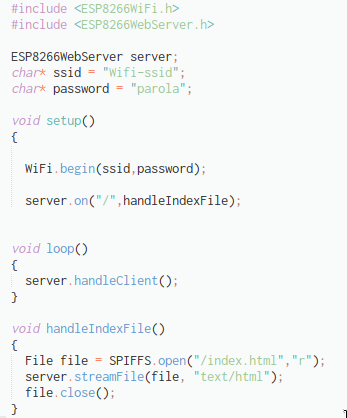
\includegraphics[width=0.7\textwidth]{gorseller/webServer}
\caption{ESP8266 ile Web Sunucu Kodları}\label{fig:webServer}
\end{figure}

Kodlarda bulunan "ssid" ve "password" değişkenleri bağlanılacak olan Wİ-Fİ ağının adını ve şifresini tutmaktadır. Bu tutulan değişkenler "WiFi.begin()" fonksiyonunda kullanılarak kablosuz ağa bağlanır. Bağlatı kurulduktan sonra "server.on("/", handleIndexFile)" satırı ile, kullanıcı tarafıdan gelen isteği "handleIndexFile" işleyici fonsiyonuna yönlendirir. Yönlendilen fonksiyon, ESP8266 dosya sistemi içerisinde bulunan "index.html" adındaki dosyayı kullanıcıya sunar.

Sunucuya bir istek yaptığında sunucu ilgili işleyici fonksionunu çağırır. İşyeci fonsiyonun isteğe bağlı olarak iki görevi üstlenmiştir. Bu görevler; ilgili dosyanın servis edilmesi ya da belirlenen betiğin çalıştırılmasıdır.

